\documentclass{article}
\usepackage{oconnor}
\usepackage{ wasysym }

%% UPDATE these variables:
\renewcommand{\hwnum}{3}
%\renewcommand{\labelitemii}[$\$][]{}
\title{CSCI 446, Project Design 03}
\author{Group 20: Jack Tetrault, John Hultman, Patrick O'Connor}
%%\date{due: 15 January 2021}

\begin{document}

\maketitle

CSCI 446 Artificial Intelligence

Project 03: Bayesian Networks and Probabilistic Inference

Elements of Design Document
\begin{enumerate}
    \item UML Class Diagram
    \item Textual Explanation of Major Classes in UML Diagram
    \item Major Design Decisions
    \item Experimental Design for Testing Results
\end{enumerate}
% ============================================
% ============================================
\nextprob{UML Class Diagram}

% ============================================

%\paragraph{Not needed for this project}


\begin{figure}
    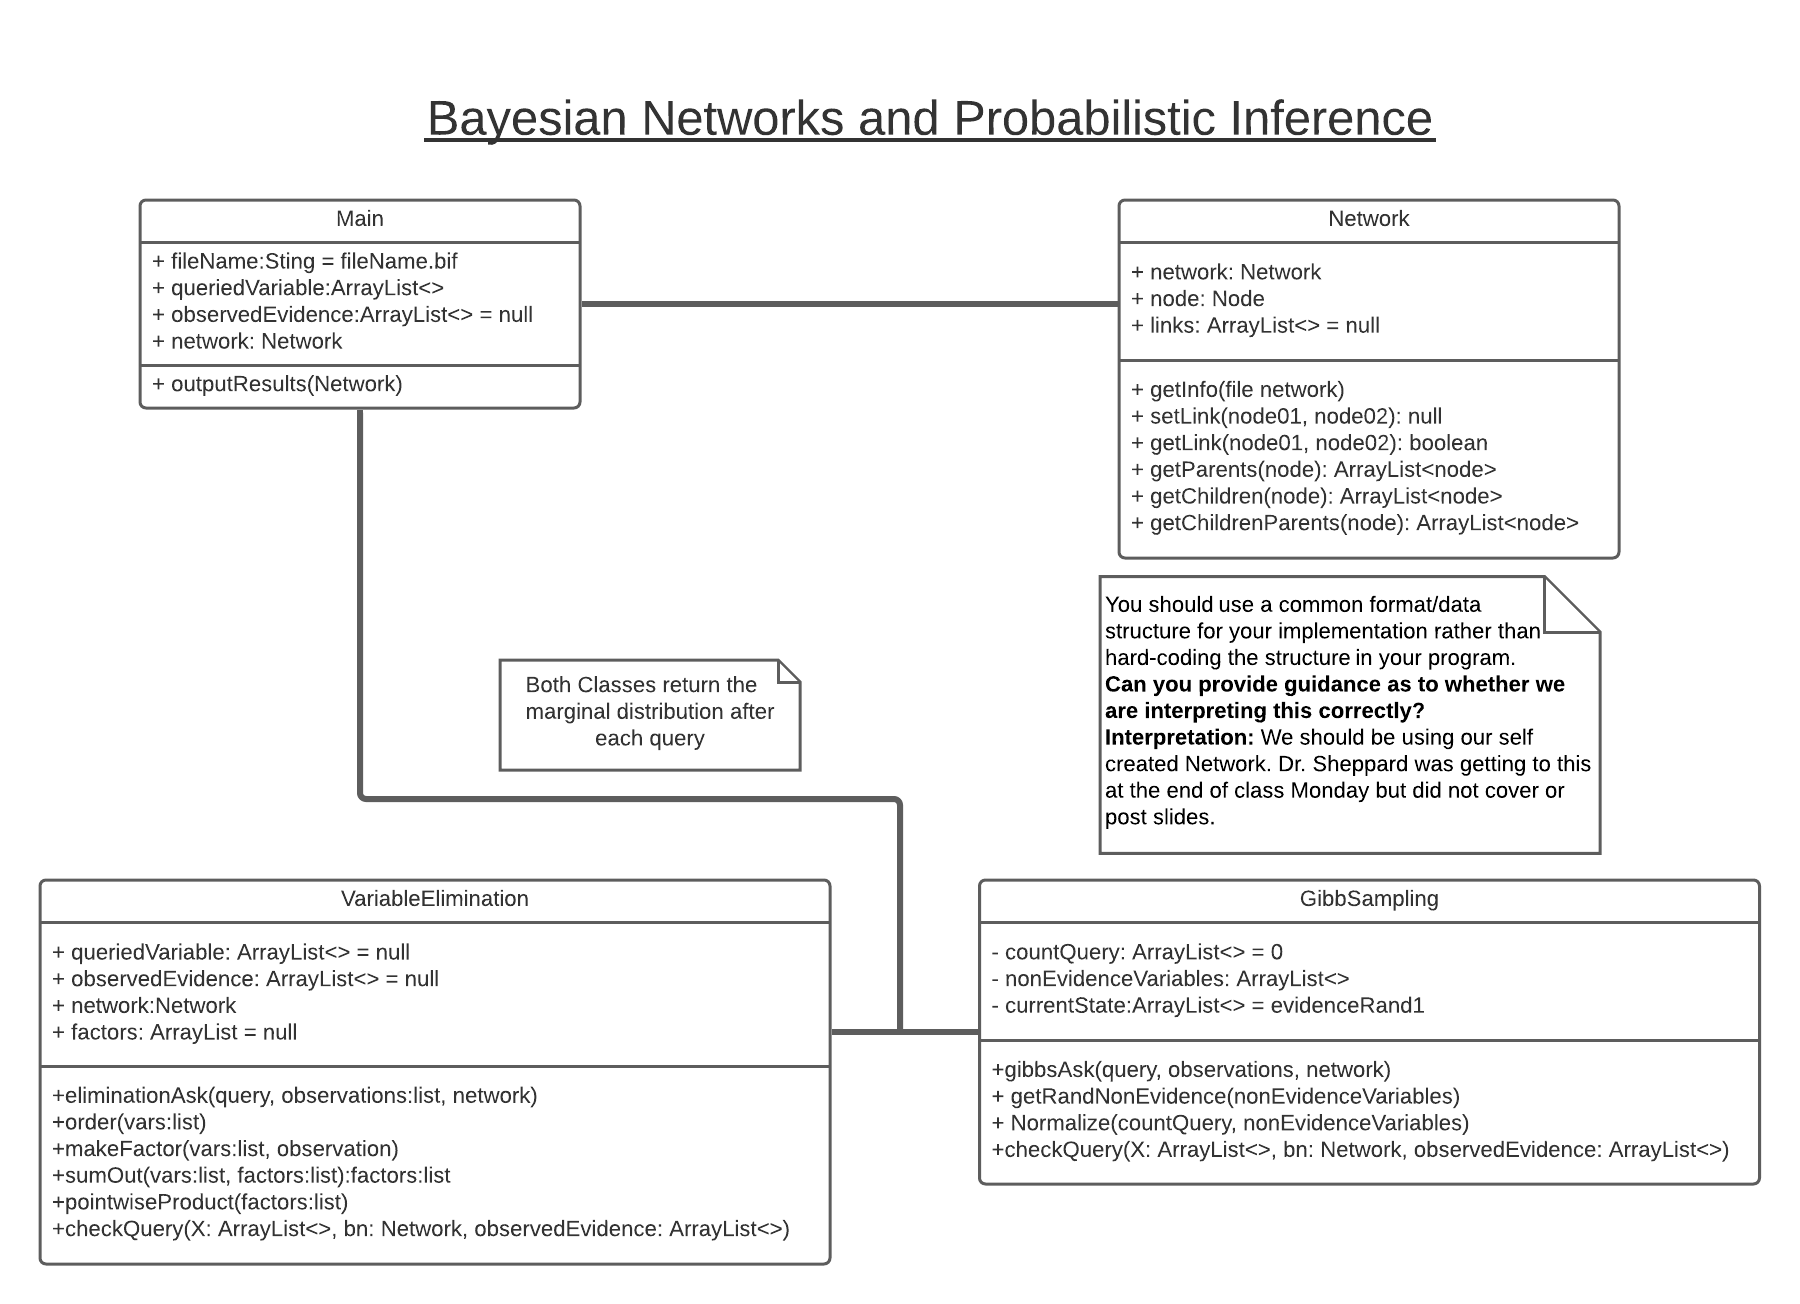
\includegraphics[width=\textwidth]{BayesUMLDiagram.png}
    \caption{UML Drawn using Lucid App}
    \label{fig:num01}
\end{figure}
See figure \ref{fig:num01} for UML Class Diagram

% ============================================
% ============================================
\nextprob{Textual Explanation of Major Classes in UML Diagram}
% ============================================

%Paste paragraphs below here
\begin{enumerate}
    \item Network: The Network class is responsible for handling the 
    networks. In order to work with the data in each network, 
    the Network class takes in a network and creates a similarly 
    formatted data structure in order to be manipulated and 
    implemented in our program.
    \item Main: The Main class is the driver for our program. 
    Here, we can import networks, set our current network, and 
    execute our distribution tests accordingly. 
    \item VariableElimination: The VariableElimination class is 
    our “exact inference” engine. This class implements the exact 
    inference algorithm and will be applied to our network data 
    structures in order to calculate probability distributions.
    \item GibbsSampling: The GibbsSampling class is our “approximate 
    inference” engine. Contrary to exact inference, this class implements 
    the algorithm for approximate inference of bayes networks. This version 
    chooses variables at random and will also be applied to our network data 
    structures to be implemented in our program.
\end{enumerate}



% ============================================
% ============================================
\nextprob{Major Design Decisions}
% ============================================

%Paste paragraphs below here
For the network's specifications, we decided 
to use the BIF formatted files provided to us. Other than that, 
there weren’t many significant design decisions that we were aware of or that were prompted by the assignment. 



% ============================================
% ============================================
\nextprob{Experimental Design for Testing Results}
% ============================================

%Paste paragraphs below here
The experimental design for testing our results will be to import a given network and then test the variable elimination algorithm against the gibbs sampling algorithm in varying conditions. We will test with with no evidence and then under the following stated evidence conditions: 

\begin{itemize} 
    \item Alarm Network 
         \begin{itemize} 
            \item Report $[HYPOVOLEMIA, LVFAILURE, ERRLOWOUTPUT]$
            \item Little Evidence: $HRBP=HIGH$; $CO=LOW$; $BP=HIGH$
            \item Moderate Evidence: $HRBP=HIGH$; $CO=LOW$; $BP=HIGH$; $HRSAT=LOW$; $HREKG=LOW$; $HISTORY=TRUE$
         \end{itemize}
    \item Child Network 
        \begin{itemize} 
            \item Report $[Disease]$
            \item Little Evidence: $LowerBodyO2=$ "$<5$”; $RUQO2=$“$\geq12$”; $CO2Report=$“$\geq7.5$”; $XrayReport=Asy/Patchy$
            \item Moderate Evidence: $LowerBodyO2=$ "$<5$”; $RUQO2=$“$\geq12$”; $CO2Report=$“$\geq7.5$”; $XrayReport=Asy/Patchy$; $GruntingReport=Yes$; $LVHReport=Yes$; $Age=$“$11-30 Days$”
        \end{itemize}
    \item Hailfinder Network 
        \begin{itemize} 
            \item Report [SatContMoist, LLIW]
            \item Little Evidence: $RSFcst=XNIL$; $N32StarFcst=XNIL$; $MountainFcst=XNIL$; $AreaMoDryAir=VeryWet$
            \item Moderate Evidence: $RSFcst=XNIL$; $N32StarFcst=XNIL$; $MountainFcst=XNIL$; $AreaMoDryAir=VeryWet$; $CombVerMo=Down$; $AreaMeso_ALS=Down$; $CurPropConv=Strong$
        \end{itemize}
    \item Insurance Network 
        \begin{itemize} 
            \item Report $[MedCost, ILiCost, PropCost]$
            \item Little Evidence: $Age=Adolescent$; $GoodStudent=False$; $SeniorTrain=False$; $DrivQuality=Poor$
            \item Moderate Evidence: $Age=Adolescent$; $GoodStudent=False$; $SeniorTrain=False$; $DrivQuality=Poor$; $MakeModel=Luxury$; $CarValue=FiftyThousand$; $DrivHistory=Zero$
        \end{itemize}
    \item Win95pts Network 
        \begin{itemize} 
            \item Report $[Problem1, Problem2, Problem3, Problem4, Problem5, Problem6]$
            \item $Problem1=No\_Output$
            \item $Problem2=Too\_Long$
            \item $Problem3=No$
            \item $Problem4=No$
            \item $Problem5=No$
            \item $Problem6=Yes$
        \end{itemize}
\end{itemize}
Once we have done this for both inference algorithms we will compare the resulting marginal distributions for both to see which achieved better performance in each situation. 




\end{document}

